\section{Fourier-Transformation}\label{k4.2.fourier}
\sectionauthor{Natalie Teplitska, Ole Fleck, (Constantin Burmeister)}
Bei der Fourier-Transformation handelt es sich um eine mathematische Methode zur Übersetzung eines Signals in ein Frequenzspektrum. Dank ihrer sehr allgemeinen und umfassenden Formulierung findet sie sowohl Anwendung in mathematischen Bereichen, aber auch in der Physik, wie beispielsweise in unserem Kurs bei der Verarbeitung von Radiosignalen.

\begin{figure}
    \centering
    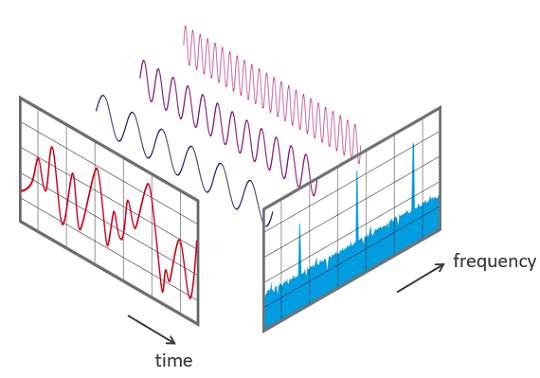
\includegraphics[width=0.6\textwidth]{k4.2/fourier.png}
    \caption{Anschauliche Darstellung der Fourier-Transformation (Quelle: www.nti-audio.com)}
    \label{k4.2.fourier.img}
\end{figure}

Ein anschauliches Beispiel ist die Spektralanalyse von Schallwellen. Die Daten (in der \cref{k4.2.fourier.img} links), die man beispielsweise mit einem Mikrofon aufnimmt, bestehen aus Schallwellen unterschiedlicher Wellenlängen. Mithilfe der Fourier-Transformation wird das Signal auf Schwingungen mit verschiedenen Wellenl\"angen aufgeteilt (in der \cref{k4.2.fourier.img} rechts), wodurch man das Frequenzspektrum erhält.

Je nachdem, welche Art von Rohdaten man erhält und welche Ausgabe erwünscht ist, nimmt die Fourier-Transformation eine leicht andere Form an.

Die kontinuierliche Fourier-Transformation (FT) benötigt als Eingabe eine Funktion, über die mit
\begin{displaymath}
\mathcal{F}(x)(s)=\int_{-\infty}^{\infty}e^{-ist}x(t)\ dt
\end{displaymath}
integriert wird. Diese Transformation lässt sich nur auf kontinuierliche Funktionen anwenden und gibt eine kontinuierliche Funktion aus.

Die diskrete Fourier-Transformation (DFT) kommt mit diskreten Werten aus und ist daher am Besten für digitale Signalverarbeitung geeignet, da die Eingabesignale meistens aus einzelnen Datenpunkten und nicht aus kontinuierlichen Funktionen bestehen. Die Formel dazu ist entsprechend kein Integral, sondern eine Summe aller gegebenen Datenpunkte: 
\begin{displaymath}
\hat a_k = \sum\limits_{j=0}^{N-1}e^{-2\pi i\cdot\frac{jk}{N}}\cdot a_j.
\end{displaymath}
Die DFT ist mit einer quadratischen Laufzeit allerdings vergleichsweise rechenintensiv. Stattdessen wird in der Signalverarbeitung meist die Fast Fourier Transformation (FFT) verwendet, welche mithilfe des \emph{Divide and Conquer} (Teile-und-Herrsche) Prinzips in der Lage ist, die Rechenzeit drastisch zu reduzieren.

Manche Probleme, welche im Wertebereich, den eigentlichen Signalen, nur durch viele komplizierte Operationen l\"osbar sind, k\"onnen im Bildbereich, dem durch die Fourier-Analyse berechneten Frequenzspektrum, mit wenigen einfachen Operationen gel\"ost werden. Dazu wendet man die Fourier-Analyse auf die Daten an, führt die notwendigen Operationen im Bildbereich aus und transformiert die Lösung zurück in den Wertebereich. Möchte man beispielsweise eine Tonaufnahme von Störsignalen bereinigen, wendet man die FFT an, löscht die unerwünschten Frequenzen im Bildbereich und übersetzt das Ergebnis zurück in Musik oder Sprache. Diese Aufgabe w\"are im Wertebereich erheblich rechenintensiver gewesen, da an einer Tonaufnahme über der Zeit nicht direkt das Störsignal ablesbar ist.

Das \enquote{Rückübersetzen} der Signale erfolgt mit der inversen (kontinuierlichen oder diskreten) Fourier-Transformation (IFT). Diese erzeugt die Funktion oder eine Menge von Datenpunkten, welche aus einem gegebenen Spektrum entsteht. Dazu werden dieselben Operationen wie bei der Berechnung des Spektrums lediglich mit anderen Faktoren angewandt.